\section{} \label{sec:2}
\quest{Perrin kísérletében (\ref{fig:1}. ábra) kolloid részecskék mozgását vizsgálták híg, vizes oldatban. A részecskék sugara $a = 0.52\ \mu m$, $\tau = 30\ s$-ként mérték a helyzetüket, s az ábrán látható négyzetrács rácsállandója $3.125\ \mu m$. Becsüljük meg a kolloid részecskék diffúziós együtthatóját kétféleképpen:
\begin{enumerate}
    \item A kezdő és a végpont közötti elmozdulásból, feltételezve, hogy a mozgás diffúziv!
    \item A $\tau$ idő alatti ugráshosszok négyzetének átlagából!
\end{enumerate}
\begin{figure}[h]
    \centering
    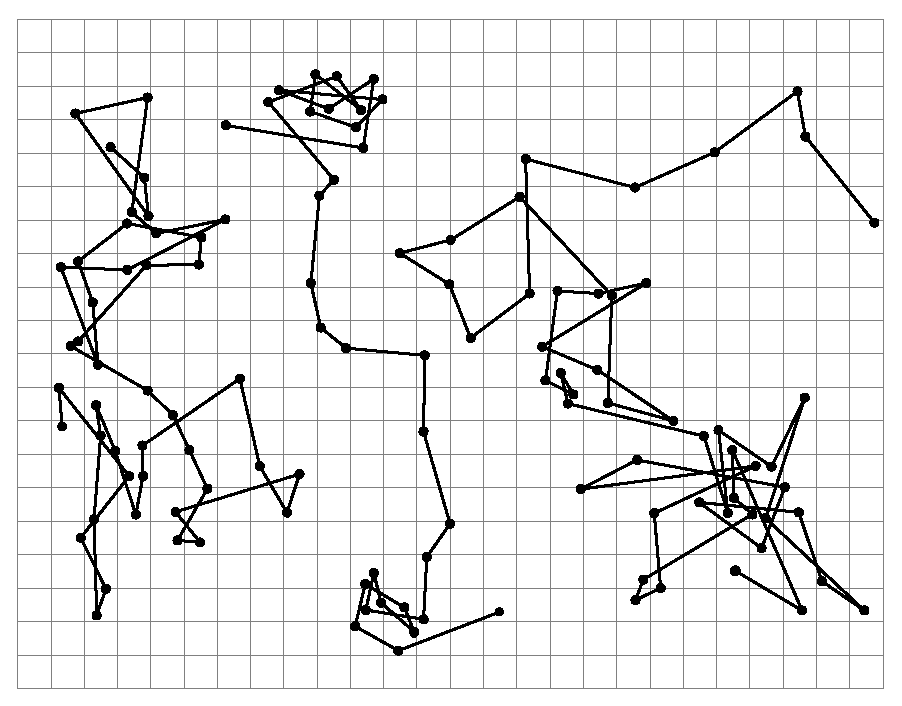
\includegraphics[width=.8\textwidth]{images/PerrinPlot.eps}
    \caption{Tracings of the motion of three colloidal particles of radius $0.52\ \mu m$ as seen under the microscope in J. Perrin’s experiments. Successive positions every $30$ seconds are joined by straight line segments. The mesh size is $3.125\ \mu m$.}
    \label{fig:1}
\end{figure}
}
\subsection{Technikai adatok}
A fenti (\ref{fig:1})-es kép Perrin kísérletét, egyik részletesen leíró 1909-es könyvéből származik\cite{perrin1909mouvement}, aminek 1910-es angol fordítása online is elérhető\cite{perrin1910brownian}. Ez az ábra \texttt{.svg}, vektorgrafikus formátumban megtalálható a Wikipédián\cite{perrinwiki}, azonban az eredetihez képest $180^{\circ}$-al elforgatott verzióban. Itt fentebb az eredeti, Perrin könyvében szereplő orientációjában illesztettem be (ahogy az a házifeladat kiírásában is szerepel). \\
A megszerzett vektorgrafikus képet Inkscape program segítségével elemeztem, ahol pontosan le tudtam mérni a $\tau$ időnként megtett lépéshosszakat, valamint a végpontok távolságát. Ezeket táblázatba rendeztem és az alábbiakban mellékeltem. \\
A rácsállandó a képen $21.53\ px$ nagyságúnak volt mérhető, a pontok távolságát ehhez arányosan mértem.

\captionof{table}{A lépéshosszak $\tau$ időközönként $px$-ben}\label{tab:1}
\begin{multicols}{2}
\begin{tabular}{||c|c|c||}
    \toprule
    \multicolumn{3}{||c||}{Lépéshosszak méretei [$px$]} \\
    \hline
    1. trajektória  & 2. trajektória  & 3. trajektória \\ \hline \hline
    70.62           & 89.01           & 29.13          \\ \hline
    28.31           & 44.65           & 24.74          \\ \hline
    65.86           & 34.60           & 80.65          \\ \hline
    55.66           & 33.98           & 47.36          \\ \hline
    72.35           & 66.46           & 74.11          \\ \hline
    86.17           & 24.61           & 20.75          \\ \hline
    47.27           & 30.99           & 45.02          \\ \hline
    36.95           & 24.00           & 70.59          \\ \hline
    37.55           & 37.18           & 42.47          \\ \hline
    33.75           & 26.73           & 66.75          \\ \hline
    52.03           & 46.72           & 40.03          \\ \hline
    86.46           & 65.03           & 27.91          \\ \hline
    68.78           & 13.81           & 39.64          \\ \hline
    43.53           & 56.28           & 48.34          \\ \hline
    58.72           & 29.14           & 17.48          \\ \hline
    38.22           & 20.80           & 33.52          \\ \hline
    78.09           & 50.71           & 65.51          \\ \hline
    31.30           & 48.80           & 5.54           \\ \hline
    26.36           & 61.37           & 56.84          \\ \hline
    57.78           & 25.90           & 22.51          \\ \hline
    19.92           & 39.94           & 24.67          \\ \hline
    15.79           & 37.38           & 27.17          \\ \hline
    20.07           & 24.30           & 38.21          \\ \hline
    89.43           & 19.65           & 14.47          \\
    \bottomrule
\end{tabular}

\begin{tabular}{||c|c|c||}
    \toprule
    \multicolumn{3}{||c||}{Lépéshosszak méretei [$px$]} \\
    \hline
    1. trajektória  & 2. trajektória  & 3. trajektória \\ \hline \hline
    51.54           & 28.26           & 25.05          \\ \hline
    53.37           & 16.94           & 82.95          \\ \hline
    41.20           & 29.12           & 25.88          \\ \hline
    48.96           & 27.74           & 34.42          \\ \hline
    81.17           & 31.66           & 57.43          \\ \hline
    86.46           & 69.58           & 75.67          \\ \hline
    32.95           &                 & 19.52          \\ \hline
    46.57           &                 & 25.05          \\ \hline
    63.96           &                 & 42.80          \\ \hline
    49.48           &                 & 31.76          \\ \hline
    41.77           &                 & 19.75          \\ \hline
    96.20           &                 & 53.63          \\ \hline
    40.61           &                 & 61.54          \\ \hline
    113.00          &                 & 17.98          \\ \hline
    71.62           &                 & 36.43          \\ \hline
    48.12           &                 & 50.16          \\ \hline
    17.83           &                 & 72.16          \\ \hline
    14.10           &                 & 24.70          \\ \hline
    81.25           &                 &                \\ \hline
    15.93           &                 &                \\ \hline
    30.56           &                 &                \\ \hline
    111.93          &                 &                \\ \hline
    49.85           &                 &                \\ \hline
                    &                 &                \\
    \bottomrule
\end{tabular}
\end{multicols}
\hfill

\begin{center}
\captionof{table}{A végpontok távolsága $px$-ben}\label{tab:2}
\begin{tabular}{||c|c|c||}
    \toprule
    \multicolumn{3}{||c||}{Végpontok távolsága [$px$]} \\
    \hline
    1. trajektória  & 2. trajektória  & 3. trajektória \\ \hline \hline
    239.92          & 357.18          & 181.30         \\
    \bottomrule
\end{tabular}
\end{center}
\newpage

Ezeket az eredményeket $\frac{1}{21.53\ px} * 3.125\ \mu m$ szorzó segítségével válthatjuk át $\mu m$ dimenziójú hosszmennyiségekké, hogy számolni tudjunk velük. Ezeket ismét két táblázatban ismertetem:

\captionof{table}{A lépéshosszak $\tau$ időközönként $\mu m$-ben}\label{tab:3}
\begin{multicols}{2}
\begin{tabular}{||c|c|c||}
    \toprule
    \multicolumn{3}{||c||}{Lépéshosszak méretei [$\mu m$]} \\
    \hline
    1. trajektória  & 2. trajektória  & 3. trajektória  \\ \hline \hline
    10.25           & 12.92           & 4.23            \\ \hline
    4.11            & 6.48            & 3.59            \\ \hline
    9.56            & 5.02            & 11.71           \\ \hline
    8.08            & 4.93            & 6.87            \\ \hline
    10.50           & 9.65            & 10.76           \\ \hline
    12.51           & 3.57            & 3.01            \\ \hline
    6.86            & 4.50            & 6.53            \\ \hline
    5.36            & 3.48            & 10.25           \\ \hline
    5.45            & 5.40            & 6.16            \\ \hline
    4.90            & 3.88            & 9.69            \\ \hline
    7.55            & 6.78            & 5.81            \\ \hline
    12.55           & 9.44            & 4.05            \\ \hline
    9.98            & 2.00            & 5.75            \\ \hline
    6.32            & 8.17            & 7.02            \\ \hline
    8.52            & 4.23            & 2.54            \\ \hline
    5.55            & 3.02            & 4.87            \\ \hline
    11.33           & 7.36            & 9.51            \\ \hline
    4.54            & 7.08            & 0.80            \\ \hline
    3.83            & 8.91            & 8.25            \\ \hline
    8.39            & 3.76            & 3.27            \\ \hline
    2.89            & 5.80            & 3.58            \\ \hline
    2.29            & 5.43            & 3.94            \\ \hline
    2.91            & 3.53            & 5.55            \\ \hline
    12.98           & 2.85            & 2.10            \\
    \bottomrule
\end{tabular}

\begin{tabular}{||c|c|c||}
    \toprule
    \multicolumn{3}{||c||}{Lépéshosszak méretei [$\mu m$]} \\
    \hline
    1. trajektória  & 2. trajektória  & 3. trajektória  \\ \hline \hline
    7.48            & 4.10            & 3.64            \\ \hline
    7.75            & 2.46            & 12.04           \\ \hline
    5.98            & 4.23            & 3.76            \\ \hline
    7.11            & 4.03            & 5.00            \\ \hline
    11.78           & 4.60            & 8.34            \\ \hline
    12.55           & 10.10           & 10.98           \\ \hline
    4.78            &                 & 2.83            \\ \hline
    6.76            &                 & 3.64            \\ \hline
    9.28            &                 & 6.21            \\ \hline
    7.18            &                 & 4.61            \\ \hline
    6.06            &                 & 2.87            \\ \hline
    13.96           &                 & 7.78            \\ \hline
    5.89            &                 & 8.93            \\ \hline
    16.40           &                 & 2.61            \\ \hline
    10.40           &                 & 5.29            \\ \hline
    6.98            &                 & 7.28            \\ \hline
    2.59            &                 & 10.47           \\ \hline
    2.05            &                 & 3.59            \\ \hline
    11.79           &                 &                 \\ \hline
    2.31            &                 &                 \\ \hline
    4.44            &                 &                 \\ \hline
    16.25           &                 &                 \\ \hline
    7.24            &                 &                 \\ \hline
                    &                 &                 \\
    \bottomrule
\end{tabular}
\end{multicols}

\begin{center}
\captionof{table}{A végpontok távolsága $\mu m$-ben.}\label{tab:4}
\begin{tabular}{||c|c|c||}
    \toprule
    \multicolumn{3}{||c||}{Végpontok távolsága [$\mu m$]} \\
    \hline
    1. trajektória  & 2. trajektória  & 3. trajektória \\ \hline \hline
    34.82           & 51.84           & 26.32          \\
    \bottomrule
\end{tabular}
\end{center}

\newpage

\subsection{Diffúziós együttható becslése}
A diffúzió Langevin-féle tárgyalása esetén végeredményben a következőket kapjuk elmozdulás négyzetének várható értékére:

\begin{equation} \label{eq:15}
    \left< r^{2} \right>
    =
    2 * \frac{k_{B} T}{6 \pi \eta a} * N * \tau
    =
    2 * D * N * \tau
\end{equation}
Ezt másképp az elmozdulások négyzetének átlagának hívjuk, amit - a fogalmak megkülönböztetése érdekében - az előzőhöz képest más módon jelölünk:
\begin{equation} \label{eq:16}
    \left< x^{2} \right>
    =
    2 * \frac{k_{B} T}{6 \pi \eta a} * N * \tau
    =
    2 * D * N * \tau
\end{equation}
Ezeket az értékeket a fenti táblázatok alapján kaphatjuk meg. Az első, (\ref{eq:15})-ös egyenletben szereplő értéket közvetlenül ki tudtuk mérni, ugyanis csak 1-1 mennyiséget kaptunk mind a 3 trajektória esetén az elmozdulások értékére. Ezek $\mu m$ hosszdimenzióval a \ref{tab:4}. táblázatban szerepelnek. Ezeknek ezután a négyzetét kell vegyük, hogy megkapjuk a becslésünket a keresett $\left< r^{2} \right>$-re vonatkozóan. \\
A (\ref{eq:16})-os egyenletben szereplő mennyiséget a \ref{tab:3}. táblázatban szereplő értékek négyzetének kiátlagolásával kaphatjuk meg. A számításokat könnyen elvégezhetjük, amire az alábbi értékeket kapjuk összesítve egy táblázatban a többi adattal együtt:

\begin{center}
\captionof{table}{Az elmozdulások négyzeteinek átlaga $\left( \mu m \right)^{2}$-ben}\label{tab:5}
\begin{tabular}{||c|c|c|c||}
    \toprule
                            & 1. trajektória  & 2. trajektória  & 3. trajektória  \\ \hline \hline
    $\left< r^{2} \right>$  & 1212.31         & 2687.73         & 692.48          \\ \hline
    $\left< x^{2} \right>$  & 73.31           & 37.84           & 43.87           \\
    \bottomrule
\end{tabular}
\end{center}
A (\ref{eq:15}) és (\ref{eq:16}) egyenletekben ismertetett összefüggésből megkaphatjuk a diffúziós együttható értékének számítási módját:

\begin{equation} \label{eq:17}
    D
    =
    \frac{k_{B} T}{6 \pi \eta a}
    =
    \frac{\left< r^{2} \right>}{2 * N * \tau}
    \approx
    \frac{\left< x^{2} \right>}{2 * N * \tau}
\end{equation}
Megfelelő mértékegységeket használva, a diffúziós együttható következő értékeit kapjuk a fenti adatok alapján:

\begin{center}
\captionof{table}{A diffúziós együttható értéke [$\frac{m^{2}}{s}$]}\label{tab:6}
\begin{tabular}{||c|c|c|c||}
    \toprule
                                             & 1. trajektória  & 2. trajektória  & 3. trajektória  \\ \hline \hline
    $D \left( \left< r^{2} \right> \right)$  & $4.30*10^{-13}$ & $1.49*10^{-12}$ & $2.75*10^{-13}$ \\ \hline
    $D \left( \left< x^{2} \right> \right)$  & $2.60*10^{-14}$ & $1.85*10^{-14}$ & $1.70*10^{-14}$ \\
    \bottomrule
\end{tabular}
\end{center}